\documentclass[aspectratio=169]{beamer}
\usepackage[utf8]{inputenc}
\usepackage[T1]{fontenc}
\usepackage{booktabs}
\usepackage{listings}
\usepackage{xcolor}
\usepackage{textcomp}
\usepackage{tikz}
\usetikzlibrary{arrows.meta,positioning,fit,backgrounds}

\usetheme[numbering=fraction,progressbar=frametitle]{metropolis}
\definecolor{faserblue}{HTML}{1F6FB2}
\setbeamercolor{palette primary}{bg=faserblue,fg=white}
\setbeamercolor{frametitle}{bg=faserblue,fg=white}
\setbeamercolor{progress bar}{fg=faserblue,bg=faserblue!20}
\setbeamercolor{alerted text}{fg=faserblue}

\definecolor{codebg}{RGB}{245,245,245}
\definecolor{mintbox}{HTML}{E0EBE5}
\lstdefinestyle{shell}{
  basicstyle=\ttfamily\footnotesize,
  backgroundcolor=\color{codebg},
  breaklines=true,
  columns=fullflexible,
  frame=single,
  rulecolor=\color{gray!40},
  showstringspaces=false,
}
\lstset{style=shell}

% ---- shared diagram styles -------------------------------------------------
\tikzset{
  box/.style={rectangle, draw=black!70, fill=white, rounded corners=2pt,
    align=center, text width=#1, minimum height=1.05cm, inner sep=6pt,
    font=\sffamily\small},
  box/.default=3.1cm,
  final/.style={box=#1, fill=mintbox, draw=black!70},
  final/.default=3.1cm,
  flow/.style={-{Stealth[length=2.4mm,width=2mm]}, line width=0.9pt, draw=black!55},
  dep/.style={-{Stealth[length=2.2mm,width=1.8mm]}, line width=0.8pt, draw=faserblue!70, dashed},
  lbl/.style={font=\itshape\scriptsize, text=black!55},
}
\newcommand{\dtag}[1]{{\ttfamily\scriptsize #1}}

\title{FASER V10}
\subtitle{Architecture \& workflow --- data pipeline, build graph, modules}
\author{Andr\'e Rubbia}
\institute{IPA Rubbia Group, ETH Z\"urich}
\date{\today}

\begin{document}

\begin{frame}
  \titlepage
\end{frame}

\begin{frame}{Outline}
  \tableofcontents
\end{frame}

\section{Data processing pipeline}

\begin{frame}{Data processing pipeline}
  \centering
  \resizebox{!}{0.72\textheight}{%
  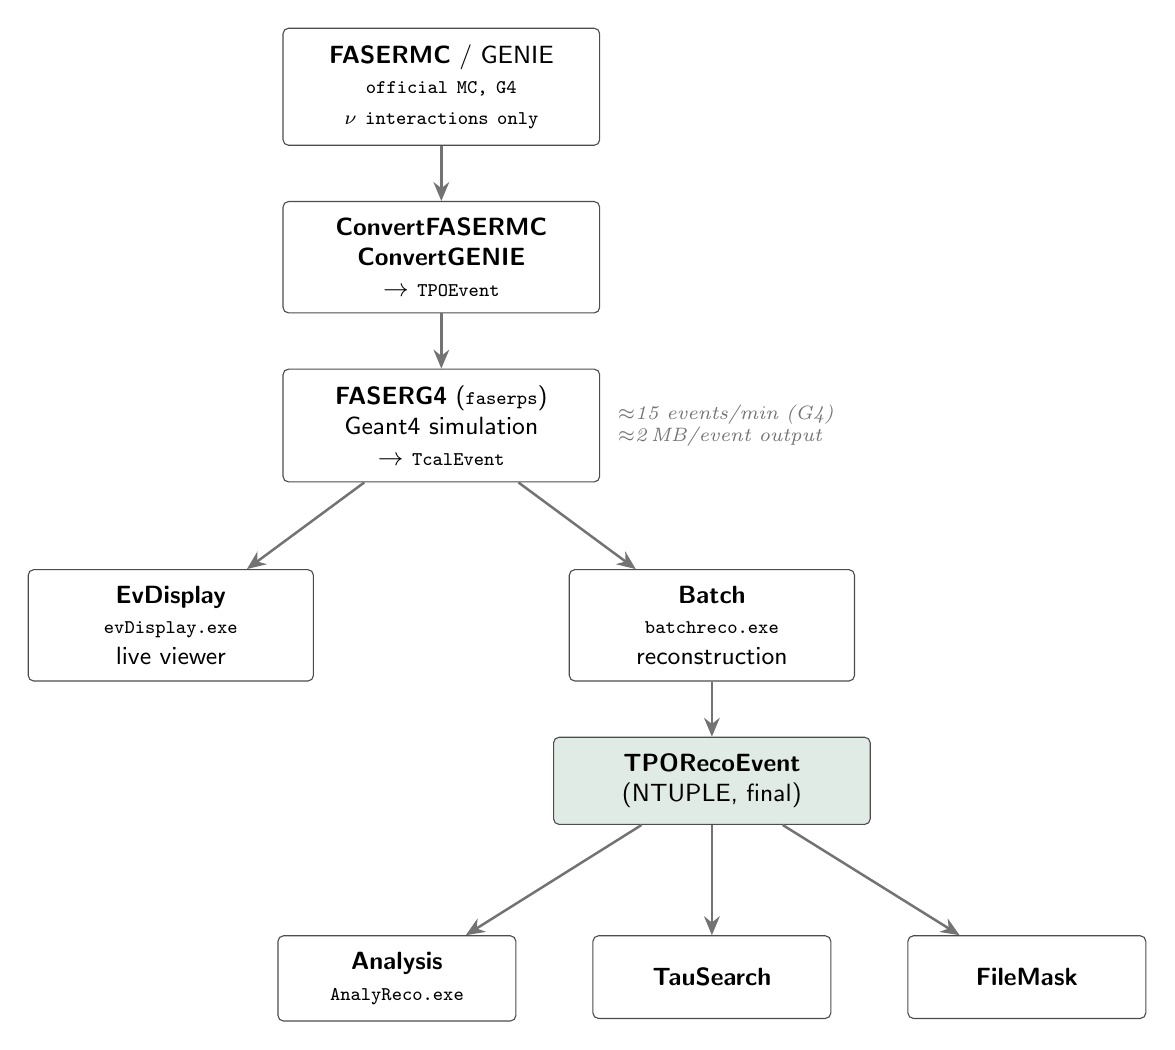
\begin{tikzpicture}[node distance=7mm and 10mm]
    \node[box=3.6cm] (mc) {\textbf{FASERMC} / GENIE\\ \dtag{official MC, G4}\\ \dtag{$\nu$ interactions only}};
    \node[box=3.6cm, below=of mc] (conv) {\textbf{ConvertFASERMC}\\ \textbf{ConvertGENIE}\\ $\rightarrow$ \dtag{TPOEvent}};
    \node[box=3.6cm, below=of conv] (g4) {\textbf{FASERG4} (\dtag{faserps})\\ Geant4 simulation\\ $\rightarrow$ \dtag{TcalEvent}};
    \node[box=3.2cm, below left=11mm and -4mm of g4] (evd) {\textbf{EvDisplay}\\ \dtag{evDisplay.exe}\\ live viewer};
    \node[box=3.2cm, below right=11mm and -4mm of g4] (batch) {\textbf{Batch}\\ \dtag{batchreco.exe}\\ reconstruction};
    \node[final=3.6cm, below=of batch] (rec) {\textbf{TPORecoEvent}\\ (NTUPLE, final)};
    \node[box=2.6cm, below=14mm of rec, xshift=-4.0cm] (ana) {\textbf{Analysis}\\ \dtag{AnalyReco.exe}};
    \node[box=2.6cm, below=14mm of rec] (tau) {\textbf{TauSearch}};
    \node[box=2.6cm, below=14mm of rec, xshift=4.0cm] (fm) {\textbf{FileMask}};

    \draw[flow] (mc) -- (conv);
    \draw[flow] (conv) -- (g4);
    \draw[flow] (g4) -- (evd);
    \draw[flow] (g4) -- (batch);
    \draw[flow] (batch) -- (rec);
    \draw[flow] (rec) -- (ana);
    \draw[flow] (rec) -- (tau);
    \draw[flow] (rec) -- (fm);

    \node[lbl, right=1mm of g4.east, text width=3.1cm] {$\approx$15 events/min (G4)\\ $\approx$2\,MB/event output};
  \end{tikzpicture}%
  }

  \vspace{2mm}
  {\scriptsize\itshape Same chain for every sample type; only the input source
  (official FASERMC or a GENIE conversion) changes which \texttt{Convert*}
  step runs.}
\end{frame}

\section{External dependency build graph}

\begin{frame}{External dependency build graph}
  \centering
  \resizebox{!}{0.72\textheight}{%
  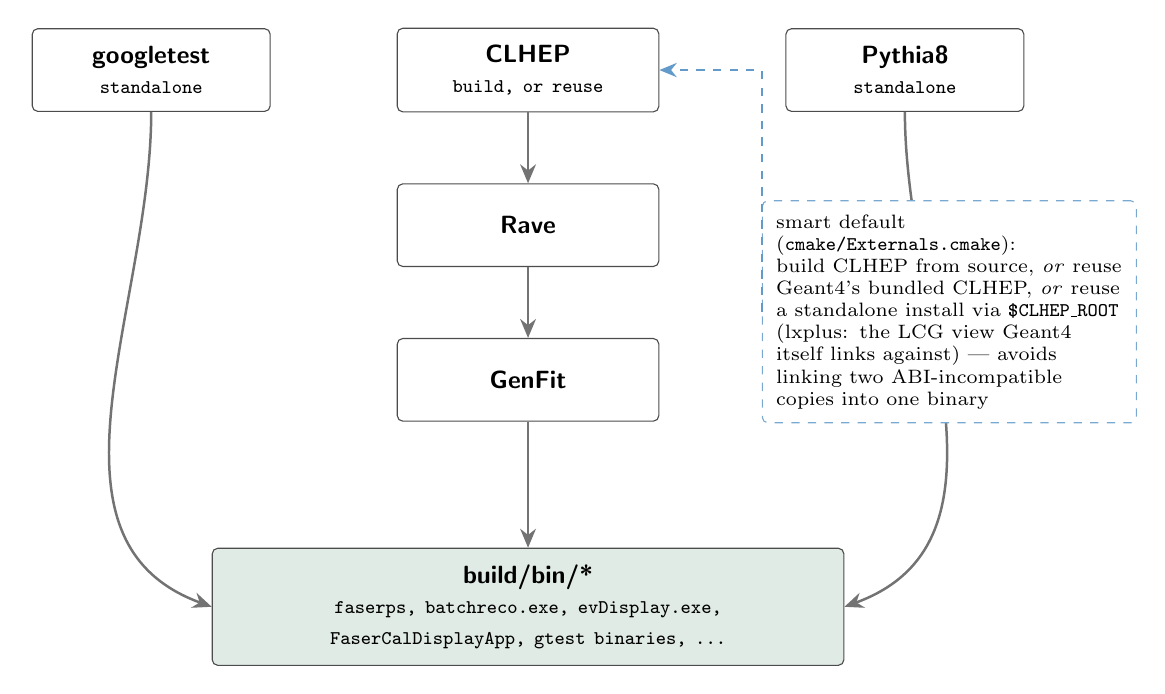
\begin{tikzpicture}[node distance=9mm and 9mm]
    \node[box=2.6cm] (gtest) {\textbf{googletest}\\ \dtag{standalone}};
    \node[box=2.9cm, right=16mm of gtest] (clhep) {\textbf{CLHEP}\\ \dtag{build, or reuse}};
    \node[box=2.6cm, right=16mm of clhep] (pythia) {\textbf{Pythia8}\\ \dtag{standalone}};

    \node[box=2.9cm, below=of clhep] (rave) {\textbf{Rave}};
    \node[box=2.9cm, below=of rave] (genfit) {\textbf{GenFit}};

    \node[final=7.6cm, below=16mm of genfit, xshift=0mm] (bin)
      {\textbf{build/bin/*}\\ \dtag{faserps, batchreco.exe, evDisplay.exe, FaserCalDisplayApp, gtest binaries, \ldots}};

    \draw[flow] (clhep) -- (rave);
    \draw[flow] (rave) -- (genfit);
    \draw[flow] (genfit.south) -- (bin.north);
    \draw[flow] (gtest.south) to[out=-90,in=160] (bin.west);
    \draw[flow] (pythia.south) to[out=-90,in=20] (bin.east);

    \node[rectangle, draw=faserblue!60, dashed, rounded corners=2pt, fill=white,
      align=left, text width=4.4cm, font=\scriptsize, right=13mm of rave,
      yshift=-11mm, inner sep=5pt] (note)
      {smart default (\texttt{cmake/Externals.cmake}): build CLHEP from
        source, \emph{or} reuse Geant4's bundled CLHEP, \emph{or} reuse a
        standalone install via \texttt{\$CLHEP\_ROOT} (lxplus: the LCG view
        Geant4 itself links against) --- avoids linking two
        ABI-incompatible copies into one binary};
    \draw[dep] (note.west) |- (clhep.east);
  \end{tikzpicture}%
  }

  \vspace{1mm}
  {\scriptsize\itshape \texttt{FASER\_BUILD\_EXTERNALS=ON} (default) builds all
  five as a CMake superbuild before configuring FASER's own packages.}
\end{frame}

\section{Repository \& module architecture}

\begin{frame}{Repository \& module architecture}
  \centering
  \resizebox{!}{0.74\textheight}{%
  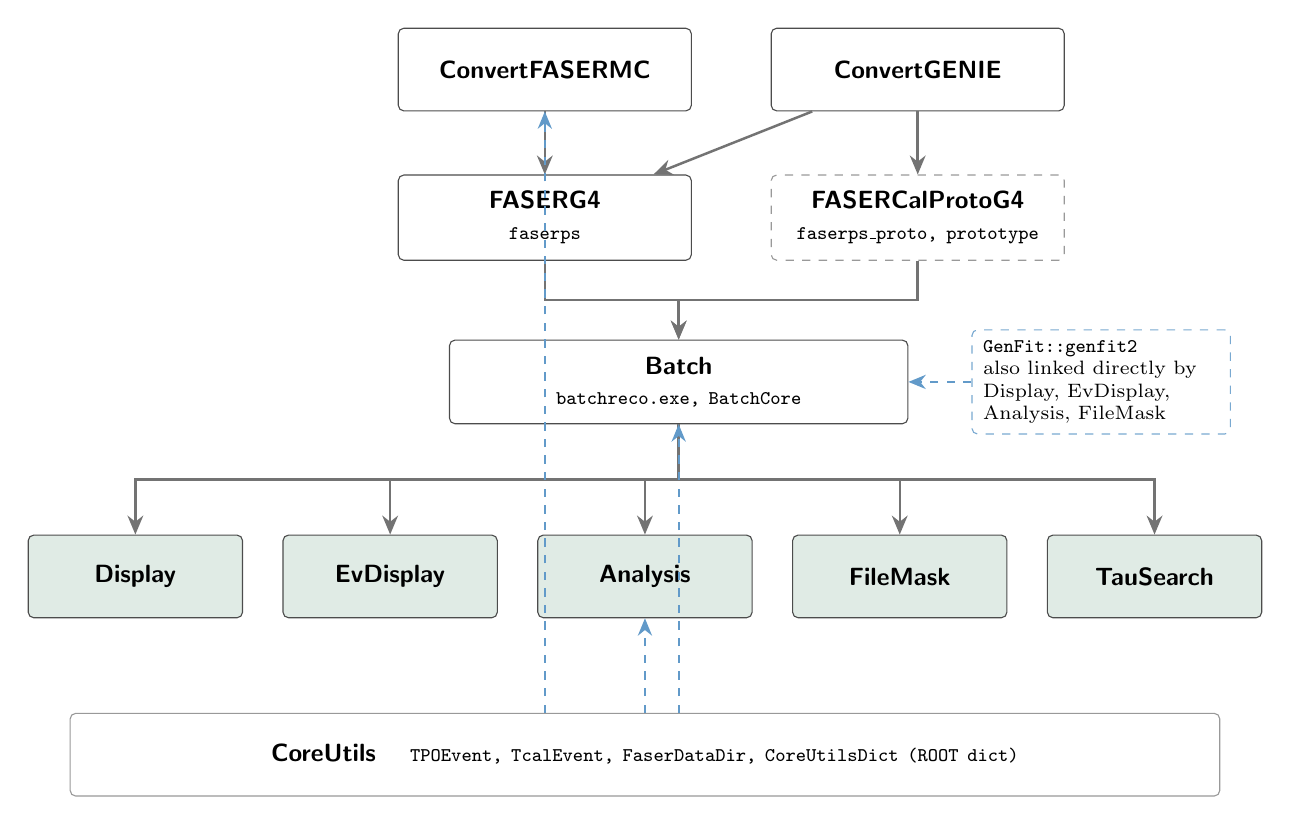
\begin{tikzpicture}[node distance=8mm and 6mm]
    \node[box=3.3cm] (cfm) {\textbf{ConvertFASERMC}};
    \node[box=3.3cm, right=10mm of cfm] (cg) {\textbf{ConvertGENIE}};

    \node[box=3.3cm, below=of cfm] (g4) {\textbf{FASERG4}\\ \dtag{faserps}};
    \node[box=3.3cm, draw=black!40, dashed, below=of cg] (protog4)
      {\textbf{FASERCalProtoG4}\\ \dtag{faserps\_proto, prototype}};

    \node[box=5.4cm, below=10mm of g4, xshift=1.7cm] (batch) {\textbf{Batch}\\ \dtag{batchreco.exe, BatchCore}};

    \node[final=2.3cm, below=14mm of batch, xshift=-6.9cm] (disp) {\textbf{Display}};
    \node[final=2.3cm, right=5mm of disp] (evd) {\textbf{EvDisplay}};
    \node[final=2.3cm, right=5mm of evd] (ana) {\textbf{Analysis}};
    \node[final=2.3cm, right=5mm of ana] (fmask) {\textbf{FileMask}};
    \node[final=2.3cm, right=5mm of fmask] (tau) {\textbf{TauSearch}};

    \node[box, draw=black!40, below=12mm of ana, minimum width=14.6cm, text width=13.8cm]
      (core) {\textbf{CoreUtils} \quad \dtag{TPOEvent, TcalEvent, FaserDataDir, CoreUtilsDict (ROOT dict)}};

    \draw[flow] (cfm) -- (g4);
    \draw[flow] (cg) -- (g4);
    \draw[flow] (cg) -- (protog4);
    \draw[flow] (g4.south) -- ++(0,-5mm) -| (batch.north);
    \draw[flow] (protog4.south) -- ++(0,-5mm) -| (batch.north);
    \draw[flow] (batch.south) -- ++(0,-7mm) -| (disp.north);
    \draw[flow] (batch.south) -- ++(0,-7mm) -| (evd.north);
    \draw[flow] (batch.south) -- ++(0,-7mm) -| (ana.north);
    \draw[flow] (batch.south) -- ++(0,-7mm) -| (fmask.north);
    \draw[flow] (batch.south) -- ++(0,-7mm) -| (tau.north);

    \draw[dep] (core.north -| cfm) -- (cfm.south);
    \draw[dep] (core.north -| batch) -- (batch.south);
    \draw[dep] (core.north -| ana) -- (ana.south);

    \node[rectangle, draw=faserblue!60, dashed, rounded corners=2pt, fill=white,
      align=left, text width=3.0cm, font=\scriptsize, right=8mm of batch,
      inner sep=4pt] (gf) {\texttt{GenFit::genfit2}\\ also linked directly by
      Display, EvDisplay, Analysis, FileMask};
    \draw[dep] (gf.west) -- (batch.east);
  \end{tikzpicture}%
  }

  \vspace{1mm}
  {\scriptsize\itshape Solid arrows: build/data flow (CMakeLists.txt
  \texttt{add\_subdirectory} order). Dashed arrows: shared-library
  dependency (\texttt{target\_link\_libraries}). Mint: user-facing leaf
  executables.}
\end{frame}

\section{Where to look}

\begin{frame}{Where to look}
  \begin{itemize}
    \item \texttt{cmake/Externals.cmake} --- the superbuild in this talk's
      second diagram: CLHEP/Rave/GenFit/googletest/Pythia8, including the
      CLHEP reuse smart-default (from-source / Geant4-bundled /
      \texttt{\$CLHEP\_ROOT})
    \item \texttt{docs/INSTALL.md} --- full CMake build: prerequisites,
      every \texttt{FASER\_BUILD\_*} option, troubleshooting a clean build
    \item \texttt{docs/GEANT4\_INSTALL.md} --- building/installing Geant4
      itself
    \item \texttt{run\_faserps.md} / \texttt{run\_batchreco.md} --- prose
      docs for the pipeline's two wrapper scripts (first diagram)
    \item \texttt{docs/REGRESSION\_TESTS.md} --- the regression suite
      (\texttt{run\_regression\_tests.py}): simulate $\to$ reconstruct
      $\to$ compare against a committed golden baseline, end to end
  \end{itemize}
\end{frame}

\end{document}
